\documentclass[12pt]{article}
\usepackage{graphicx}
\usepackage{amsmath}
\usepackage{booktabs}
\usepackage{caption}
\usepackage{hyperref}
\usepackage{float}

\title{Supplementary Material: Modeling the Interferon Response to Avian Influenza}
\author{Arjan Suri, Sahaj Satani, Hana M. Dobrovolny}
\date{January 2026}

\begin{document}
\maketitle

\section*{Overview}
This supplementary document contains detailed parameter estimates and corner plots (parameter distribution visualizations) from bootstrap analyses for Model 3 (Refractory State Model) fitted to viral load and interferon data across three influenza virus strains in both nasal and tracheal tissues. Model 3 was identified as the best-performing model, assuming interferon moves target cells into a temporary refractory state where they are protected from infection.

\tableofcontents
\newpage

%%%%%%%%%%%%%%%%%%%%%%%%%%%%%%%%%%%%%%%%%%%%%%%%%%%%%%%%%%%%%%%%%%%%%%%
\section{Model 3: Refractory State Model - Parameter Estimates}
%%%%%%%%%%%%%%%%%%%%%%%%%%%%%%%%%%%%%%%%%%%%%%%%%%%%%%%%%%%%%%%%%%%%%%%

The refractory state model is described by the following system of differential equations:
\begin{align*}
\frac{dT}{dt} &= -\beta TV - \gamma TF\\
\frac{dR}{dt} &= \gamma TF - \rho R\\
\frac{dI}{dt} &= \beta TV - \delta I\\
\frac{dV}{dt} &= pI - cV\\
\frac{dF}{dt} &= I - \alpha F
\end{align*}

where:
\begin{itemize}
    \item $\beta$ = infection rate (day$^{-1}$)
    \item $\delta$ = infected cell death rate (day$^{-1}$)
    \item $p$ = virus production rate (arbitrary units $\cdot$ day$^{-1}$)
    \item $c$ = virus clearance rate (day$^{-1}$)
    \item $\gamma$ = rate of transition to refractory state (day$^{-1}$)
    \item $\rho$ = rate of return from refractory state (day$^{-1}$)
    \item $\alpha$ = interferon clearance rate (day$^{-1}$)
\end{itemize}

\newpage
%------------------------------------------------------------------
\subsection{H3N2 (2003) - Nasal Tissue}
%------------------------------------------------------------------

\subsubsection{Parameter Estimates}
\begin{table}[H]
\centering
\caption{Bootstrap parameter estimates for H3N2$_{2003}$ nasal tissue (Model 3). Values represent mean estimates with 95\% confidence intervals from 1000 bootstrap resamples.}
\begin{tabular}{lccc}
\toprule
\textbf{Parameter} & \textbf{Mean} & \textbf{95\% CI Lower} & \textbf{95\% CI Upper} \\
\midrule
$\beta$ & 6.2136 & 0.1860 & 10.0000 \\
$\delta$ & 0.0009 & $<$0.0001 & $<$0.0001 \\
$p$ & 6.1344 & $<$0.0001 & 10.0000 \\
$c$ & 0.0178 & $<$0.0001 & 0.0433 \\
$\gamma$ & 0.1820 & 0.1148 & 0.2898 \\
$\rho$ & 0.0057 & $<$0.0001 & 0.0316 \\
$\alpha$ & 0.0235 & 0.0037 & 0.0462 \\
\bottomrule
\end{tabular}
\label{tab:h3n2_2003_nasal_params}
\end{table}

\subsubsection{Parameter Distribution Corner Plot}
\begin{figure}[H]
\centering
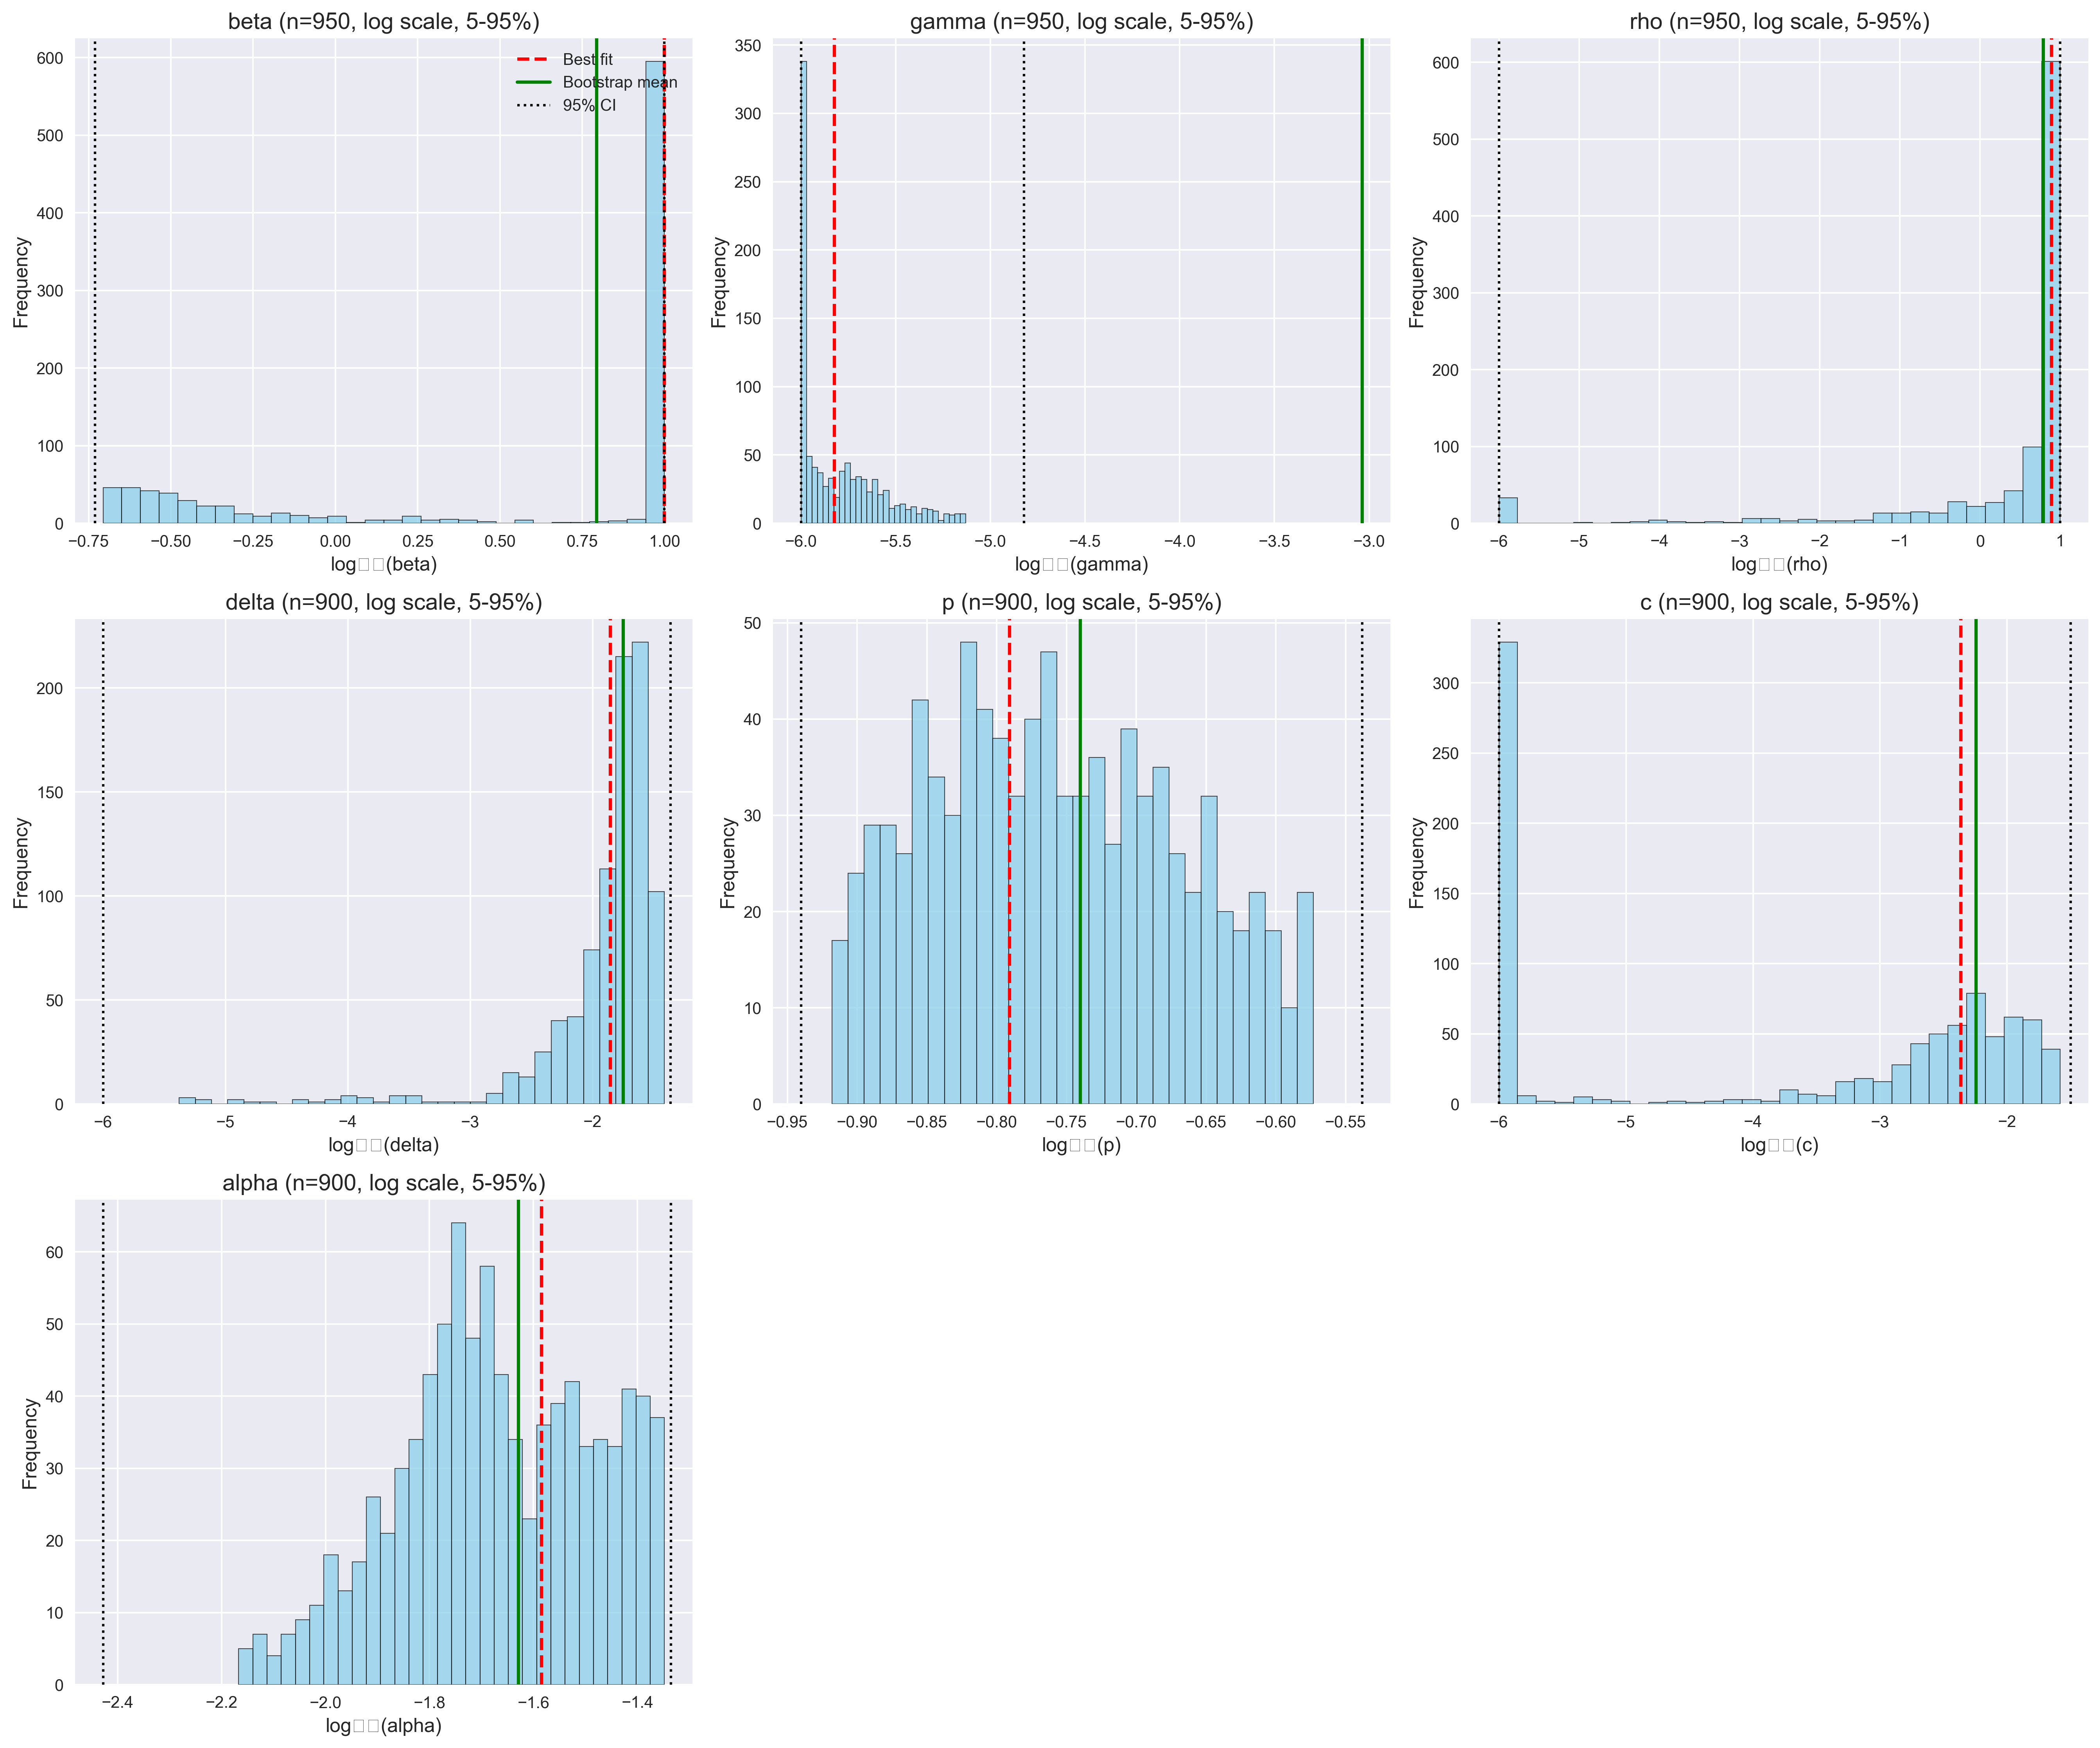
\includegraphics[width=\textwidth]{Plots/h3n2(2003)/nasal/bootstrap_results/h3n2(2003)_nasal_param_distributions.png}
\caption{Corner plot showing bootstrap parameter distributions for H3N2$_{2003}$ nasal tissue (Model 3). Diagonal panels show individual parameter distributions; off-diagonal panels show pairwise parameter correlations.}
\label{fig:h3n2_2003_nasal_corner}
\end{figure}

\newpage
%------------------------------------------------------------------
\subsection{H3N2 (2003) - Tracheal Tissue}
%------------------------------------------------------------------

\subsubsection{Parameter Estimates}
\begin{table}[H]
\centering
\caption{Bootstrap parameter estimates for H3N2$_{2003}$ tracheal tissue (Model 3). Values represent mean estimates with 95\% confidence intervals from 1000 bootstrap resamples.}
\begin{tabular}{lccc}
\toprule
\textbf{Parameter} & \textbf{Mean} & \textbf{95\% CI Lower} & \textbf{95\% CI Upper} \\
\midrule
$\beta$ & 0.0281 & 0.0141 & 0.0565 \\
$\delta$ & 0.0049 & $<$0.0001 & 0.0167 \\
$p$ & 1.0085 & $<$0.0001 & 9.7445 \\
$c$ & 0.0061 & $<$0.0001 & 0.0123 \\
$\gamma$ & 30.6946 & 1.3044 & 123.7112 \\
$\rho$ & 3.0433 & 0.1146 & 10.0000 \\
$\alpha$ & 0.0220 & 0.0049 & 0.0441 \\
\bottomrule
\end{tabular}
\label{tab:h3n2_2003_tracheal_params}
\end{table}

\subsubsection{Parameter Distribution Corner Plot}
\begin{figure}[H]
\centering
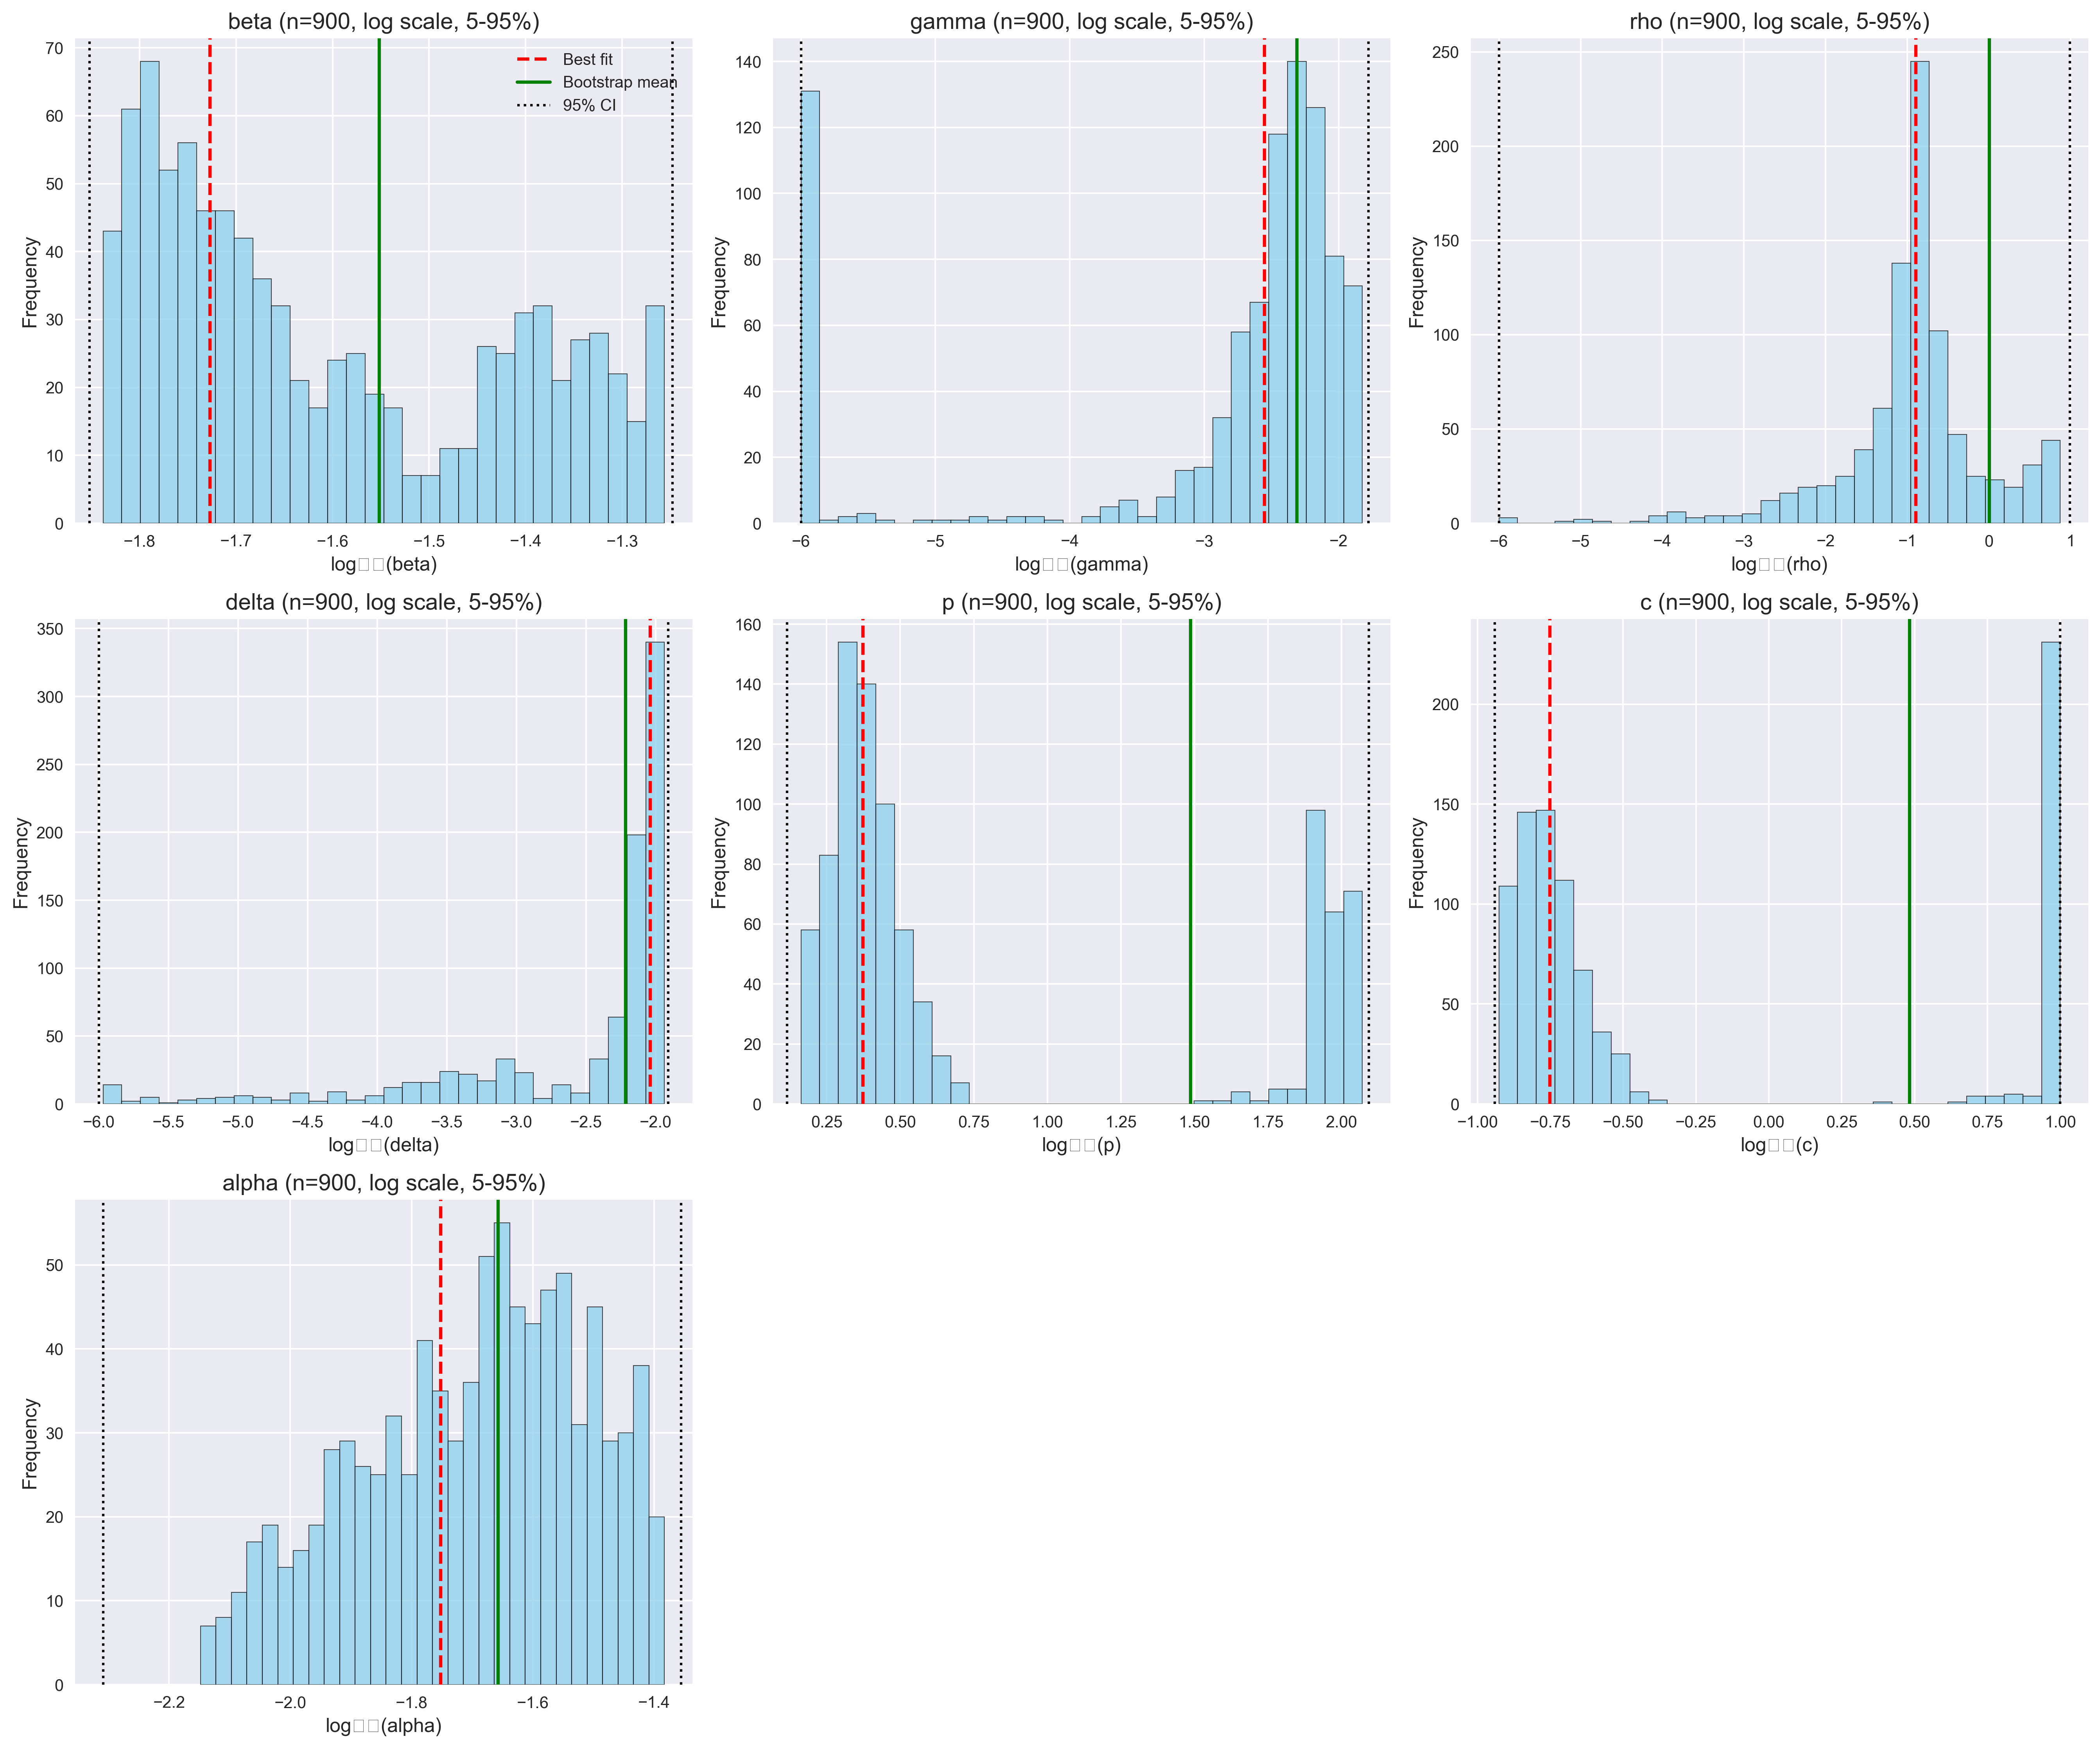
\includegraphics[width=\textwidth]{Plots/h3n2(2003)/tracheal/bootstrap_results/h3n2(2003)_tracheal_param_distributions.png}
\caption{Corner plot showing bootstrap parameter distributions for H3N2$_{2003}$ tracheal tissue (Model 3). Note the substantially higher $\gamma$ value compared to nasal tissue, indicating faster transition to refractory state in tracheal tissue.}
\label{fig:h3n2_2003_tracheal_corner}
\end{figure}

\newpage
%------------------------------------------------------------------
\subsection{H5N1 (2005) - Nasal Tissue}
%------------------------------------------------------------------

\subsubsection{Parameter Estimates}
\begin{table}[H]
\centering
\caption{Bootstrap parameter estimates for H5N1$_{2005}$ nasal tissue (Model 3). Values represent mean estimates with 95\% confidence intervals from 1000 bootstrap resamples.}
\begin{tabular}{lccc}
\toprule
\textbf{Parameter} & \textbf{Mean} & \textbf{95\% CI Lower} & \textbf{95\% CI Upper} \\
\midrule
$\beta$ & 0.6318 & 0.1401 & 5.6995 \\
$\delta$ & 0.0808 & $<$0.0001 & 1.0240 \\
$p$ & $<$0.0001 & $<$0.0001 & $<$0.0001 \\
$c$ & 0.0137 & 0.0050 & 0.0397 \\
$\gamma$ & 0.2633 & 0.1358 & 0.6254 \\
$\rho$ & 0.0449 & 0.0096 & 0.1286 \\
$\alpha$ & 0.0461 & 0.0148 & 0.0646 \\
\bottomrule
\end{tabular}
\label{tab:h5n1_2005_nasal_params}
\end{table}

\subsubsection{Parameter Distribution Corner Plot}
\begin{figure}[H]
\centering
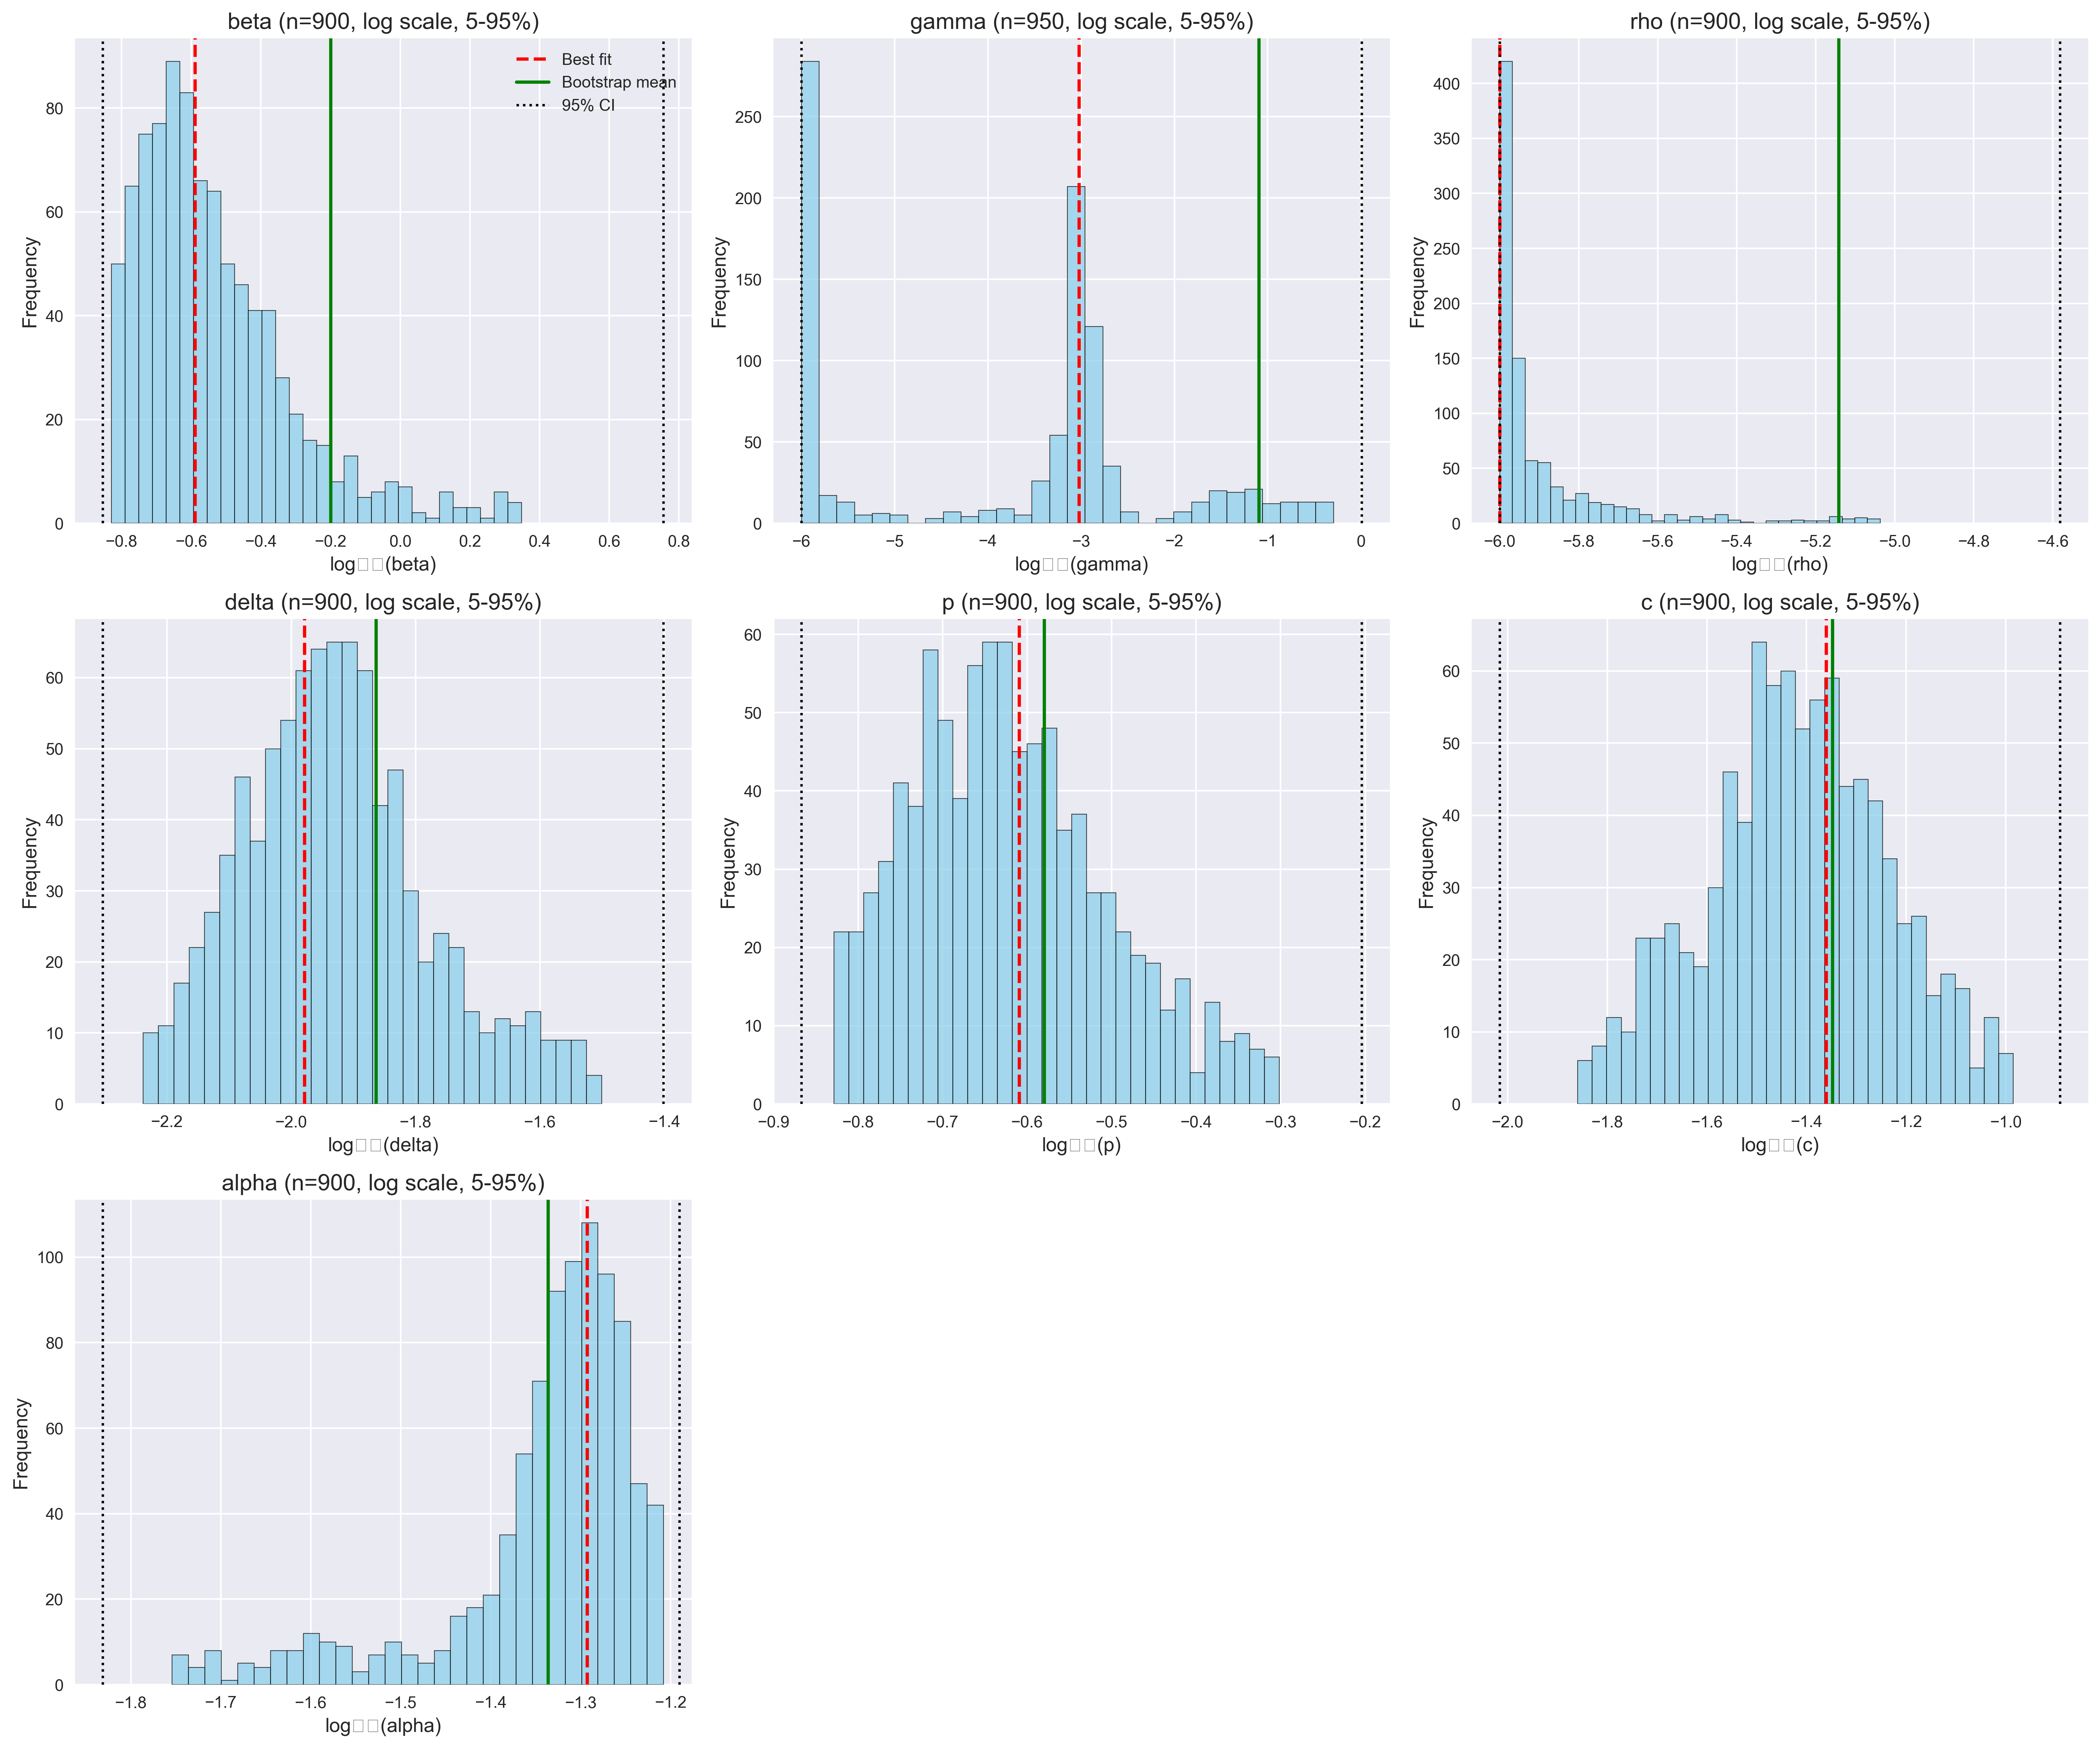
\includegraphics[width=\textwidth]{Plots/h5n1(2005)/nasal/bootstrap_results/h5n1(2005)_nasal_param_distributions.png}
\caption{Corner plot showing bootstrap parameter distributions for H5N1$_{2005}$ nasal tissue (Model 3).}
\label{fig:h5n1_2005_nasal_corner}
\end{figure}

\newpage
%------------------------------------------------------------------
\subsection{H5N1 (2005) - Tracheal Tissue}
%------------------------------------------------------------------

\subsubsection{Parameter Estimates}
\begin{table}[H]
\centering
\caption{Bootstrap parameter estimates for H5N1$_{2005}$ tracheal tissue (Model 3). Values represent mean estimates with 95\% confidence intervals from 1000 bootstrap resamples.}
\begin{tabular}{lccc}
\toprule
\textbf{Parameter} & \textbf{Mean} & \textbf{95\% CI Lower} & \textbf{95\% CI Upper} \\
\midrule
$\beta$ & 0.0905 & 0.0054 & 1.2094 \\
$\delta$ & 0.6269 & $<$0.0001 & 9.9996 \\
$p$ & 0.3292 & $<$0.0001 & 6.9327 \\
$c$ & 0.0191 & $<$0.0001 & 0.0998 \\
$\gamma$ & 0.2910 & 0.1000 & 1.0210 \\
$\rho$ & 0.0004 & $<$0.0001 & 0.0026 \\
$\alpha$ & 0.0504 & $<$0.0001 & 0.1239 \\
\bottomrule
\end{tabular}
\label{tab:h5n1_2005_tracheal_params}
\end{table}

\subsubsection{Parameter Distribution Corner Plot}
\begin{figure}[H]
\centering
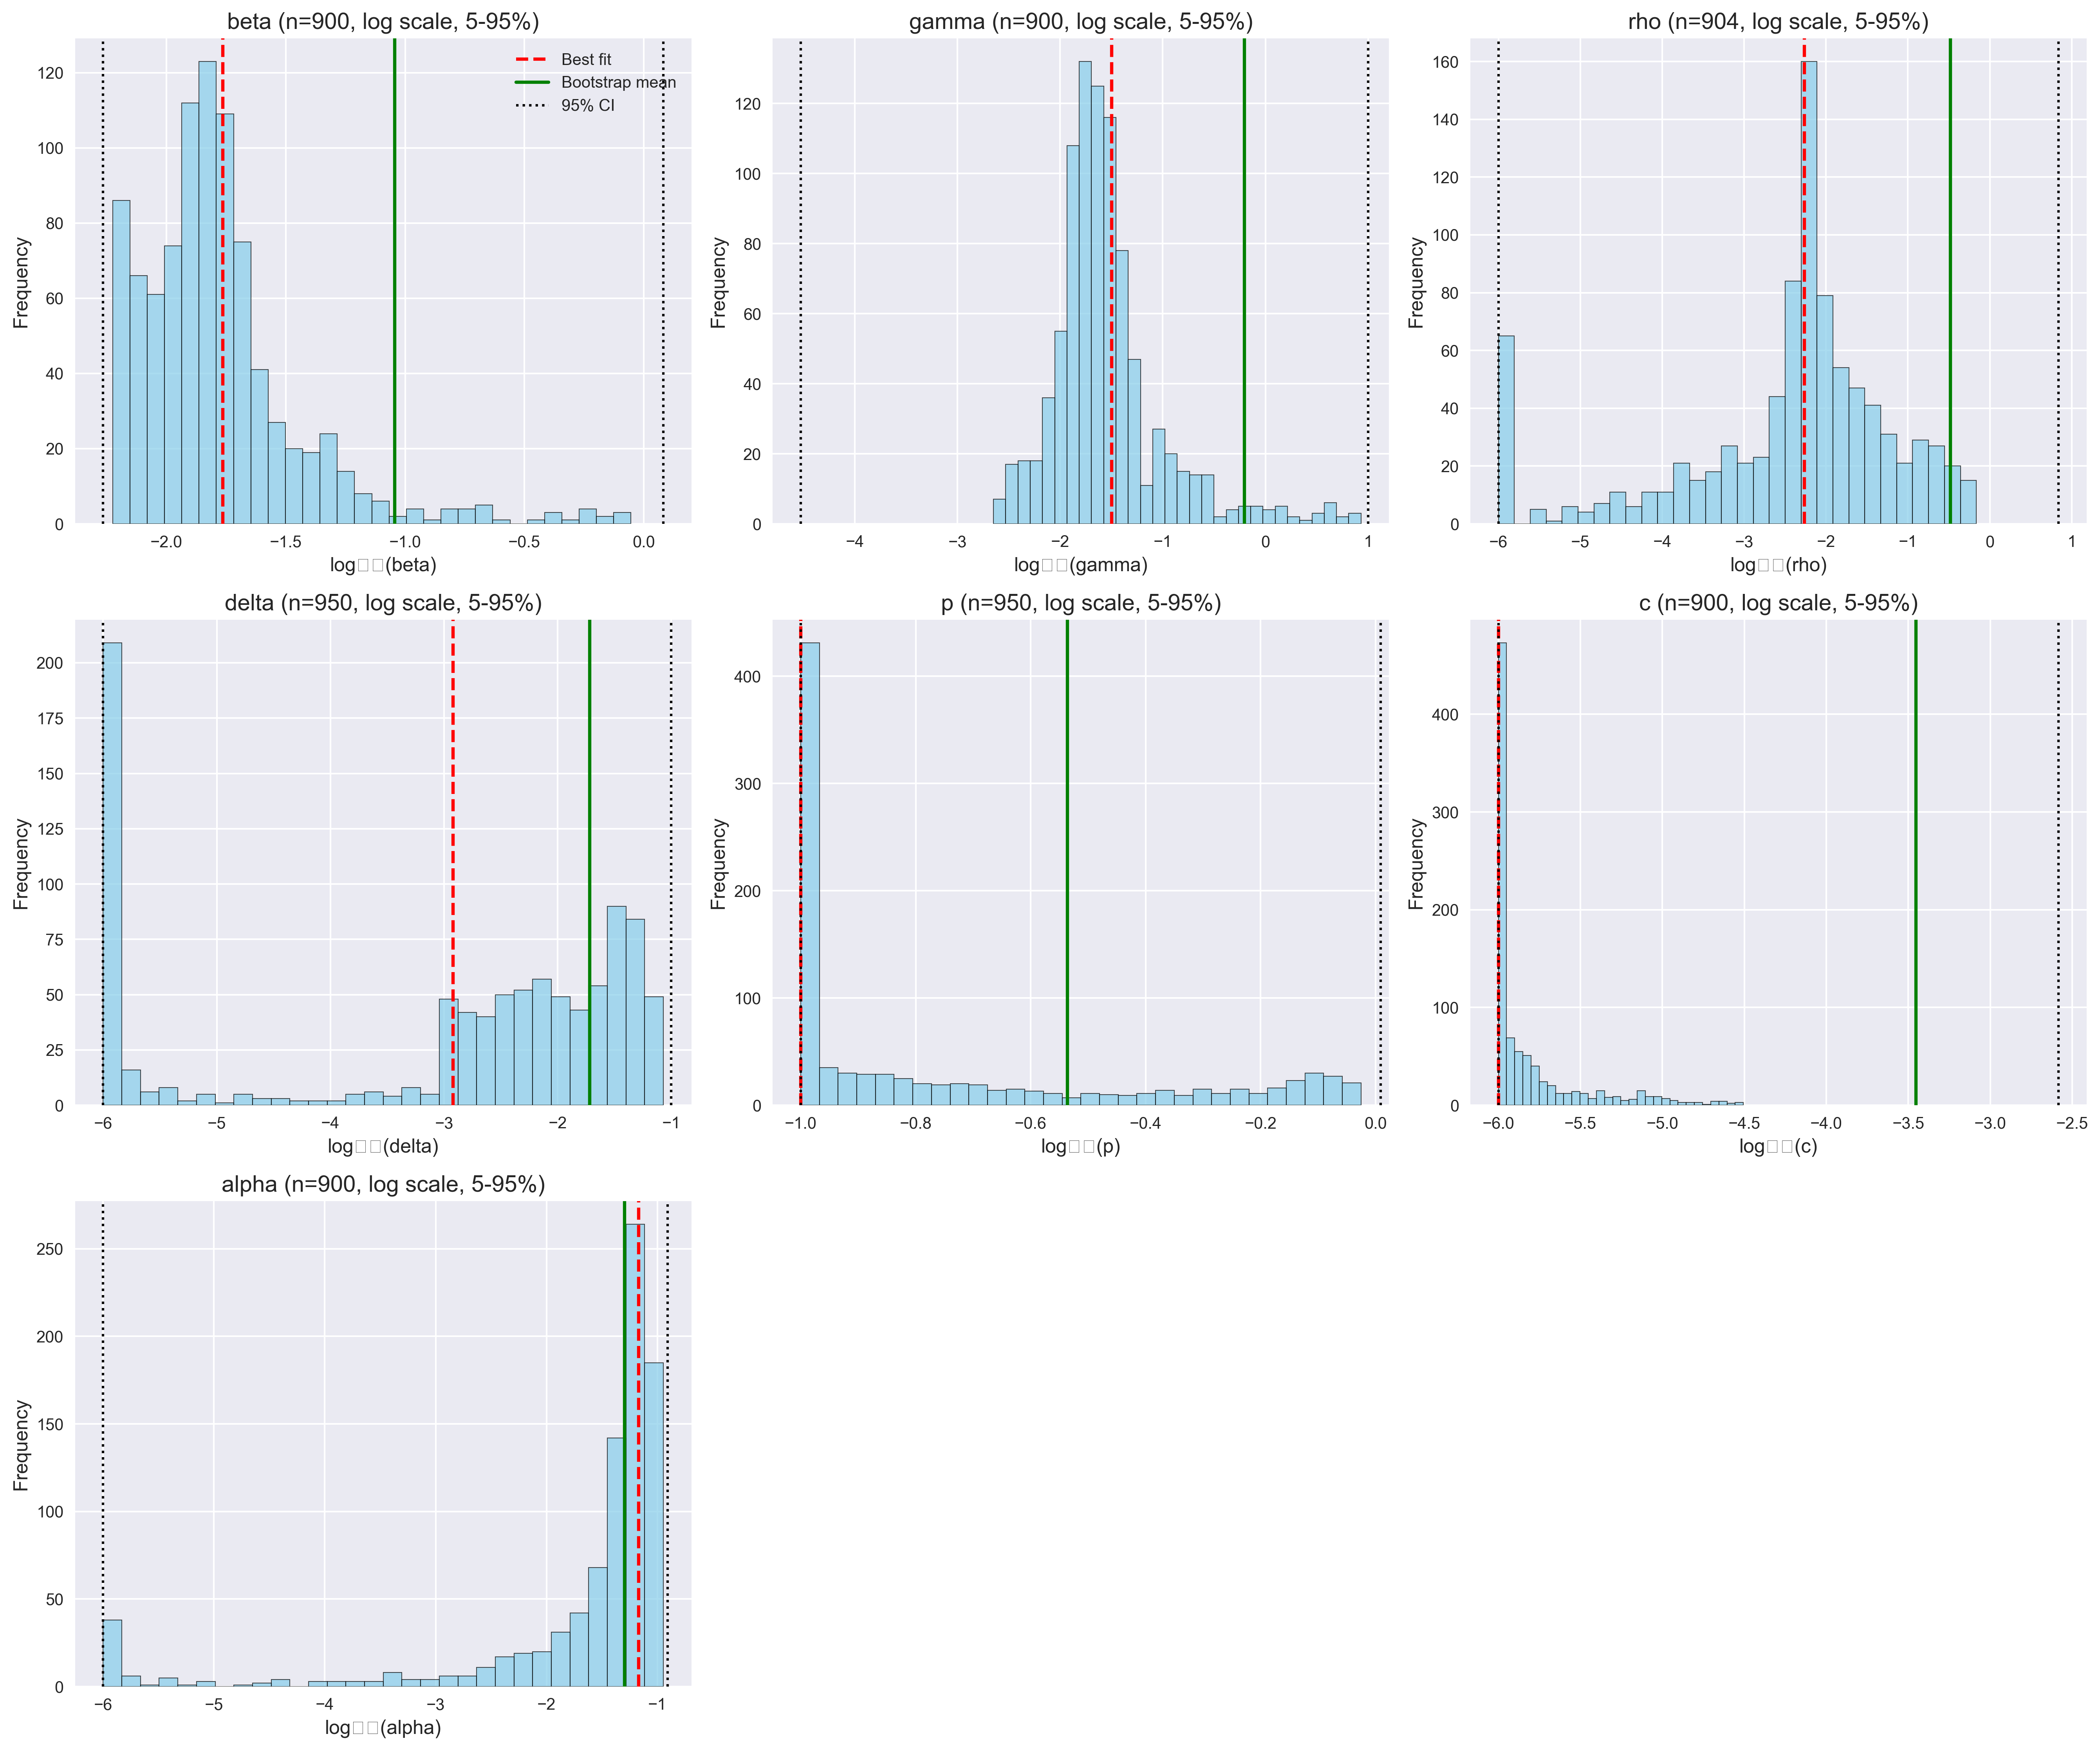
\includegraphics[width=\textwidth]{Plots/h5n1(2005)/tracheal/bootstrap_results/h5n1(2005)_tracheal_param_distributions.png}
\caption{Corner plot showing bootstrap parameter distributions for H5N1$_{2005}$ tracheal tissue (Model 3).}
\label{fig:h5n1_2005_tracheal_corner}
\end{figure}

\newpage
%------------------------------------------------------------------
\subsection{H5N1 (2022) - Nasal Tissue}
%------------------------------------------------------------------

\subsubsection{Parameter Estimates}
\begin{table}[H]
\centering
\caption{Bootstrap parameter estimates for H5N1$_{2022}$ nasal tissue (Model 3). Values represent mean estimates with 95\% confidence intervals from 1000 bootstrap resamples.}
\begin{tabular}{lccc}
\toprule
\textbf{Parameter} & \textbf{Mean} & \textbf{95\% CI Lower} & \textbf{95\% CI Upper} \\
\midrule
$\beta$ & 7.5923 & 0.2427 & 10.0000 \\
$\delta$ & 0.0014 & $<$0.0001 & 0.0001 \\
$p$ & 7.4064 & $<$0.0001 & 10.0000 \\
$c$ & 0.0294 & 0.0049 & 0.0623 \\
$\gamma$ & 0.1210 & 0.1000 & 0.2044 \\
$\rho$ & 0.0045 & $<$0.0001 & 0.0145 \\
$\alpha$ & 0.0202 & 0.0012 & 0.0459 \\
\bottomrule
\end{tabular}
\label{tab:h5n1_2022_nasal_params}
\end{table}

\subsubsection{Parameter Distribution Corner Plot}
\begin{figure}[H]
\centering
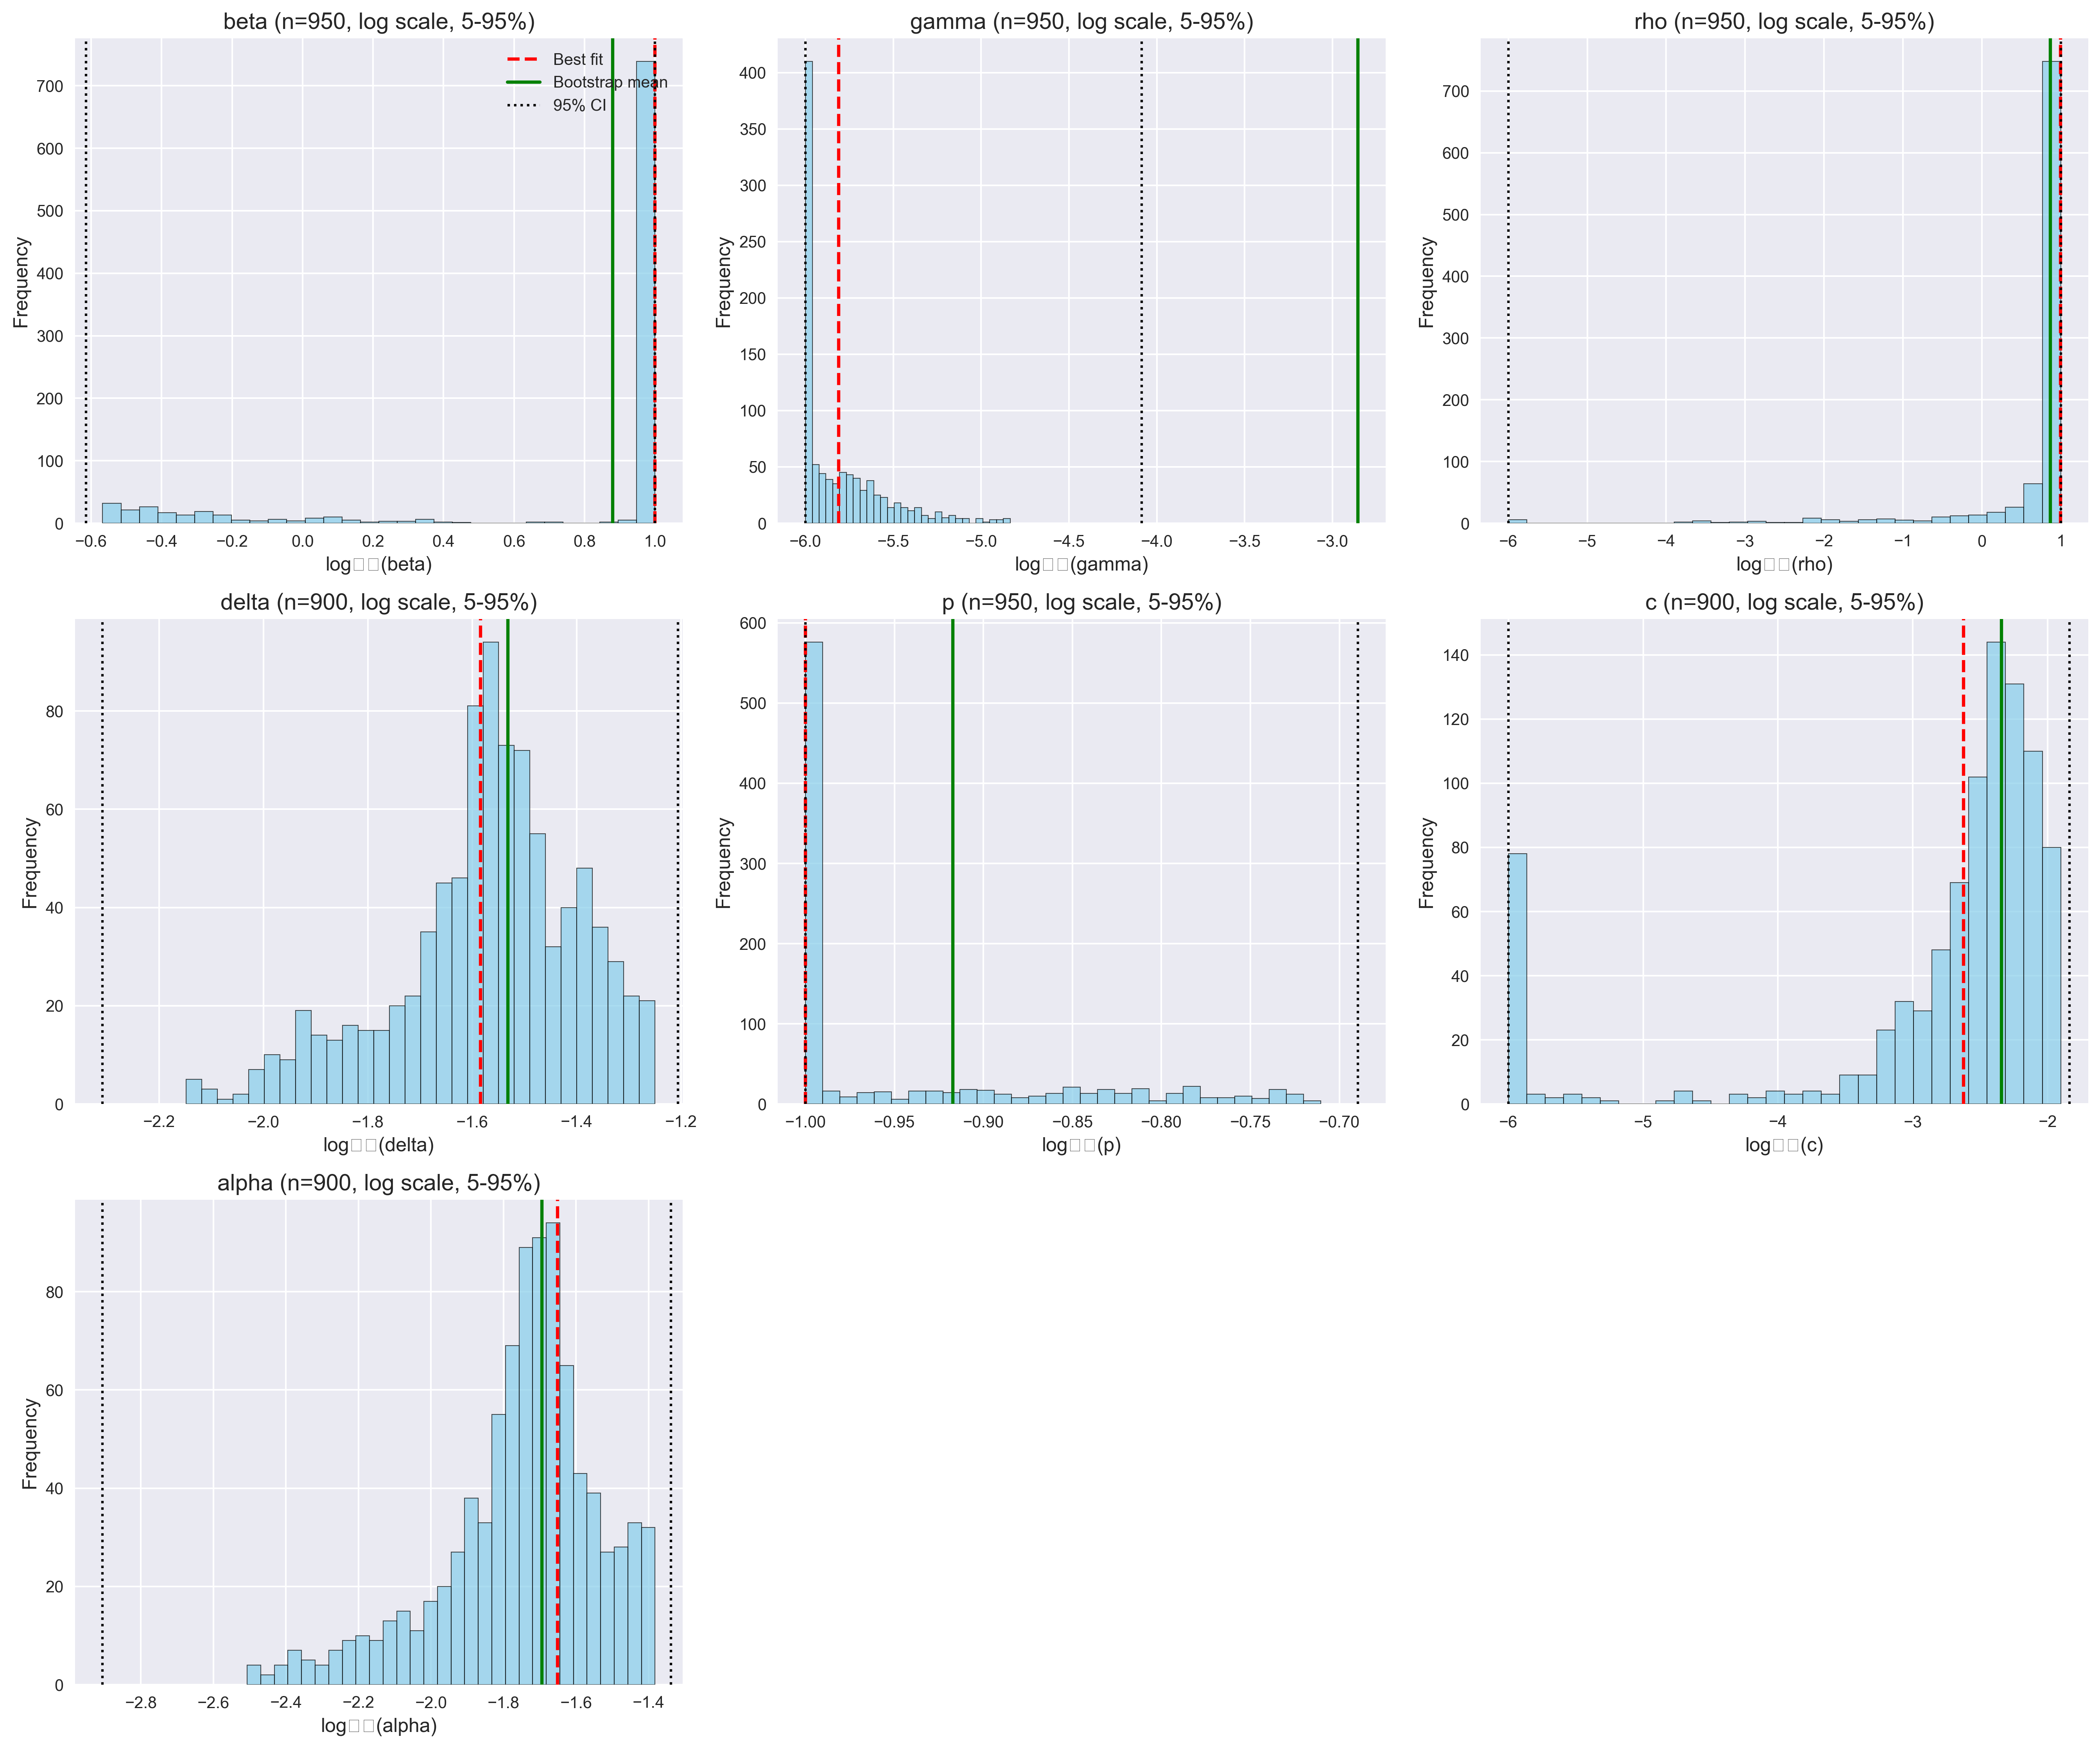
\includegraphics[width=\textwidth]{Plots/h5n1(2022)/nasal/bootstrap_results/h5n1(2022)_nasal_param_distributions.png}
\caption{Corner plot showing bootstrap parameter distributions for H5N1$_{2022}$ nasal tissue (Model 3).}
\label{fig:h5n1_2022_nasal_corner}
\end{figure}

\newpage
%------------------------------------------------------------------
\subsection{H5N1 (2022) - Tracheal Tissue}
%------------------------------------------------------------------

\subsubsection{Parameter Estimates}
\begin{table}[H]
\centering
\caption{Bootstrap parameter estimates for H5N1$_{2022}$ tracheal tissue (Model 3). Values represent mean estimates with 95\% confidence intervals from 1000 bootstrap resamples. As discussed in the main text, this dataset exhibited numerical challenges during bootstrap analysis.}
\begin{tabular}{lccc}
\toprule
\textbf{Parameter} & \textbf{Mean} & \textbf{95\% CI Lower} & \textbf{95\% CI Upper} \\
\midrule
$\beta$ & 1.5546 & 0.0384 & 10.0000 \\
$\delta$ & 0.0211 & $<$0.0001 & 0.0025 \\
$p$ & 0.8904 & $<$0.0001 & 10.0000 \\
$c$ & 0.0005 & $<$0.0001 & 0.0065 \\
$\gamma$ & 0.7282 & 0.1682 & 1.0144 \\
$\rho$ & 0.0926 & 0.0093 & 0.1286 \\
$\alpha$ & 0.0427 & 0.0267 & 0.0511 \\
\bottomrule
\end{tabular}
\label{tab:h5n1_2022_tracheal_params}
\end{table}

\subsubsection{Parameter Distribution Corner Plot}
\begin{figure}[H]
\centering
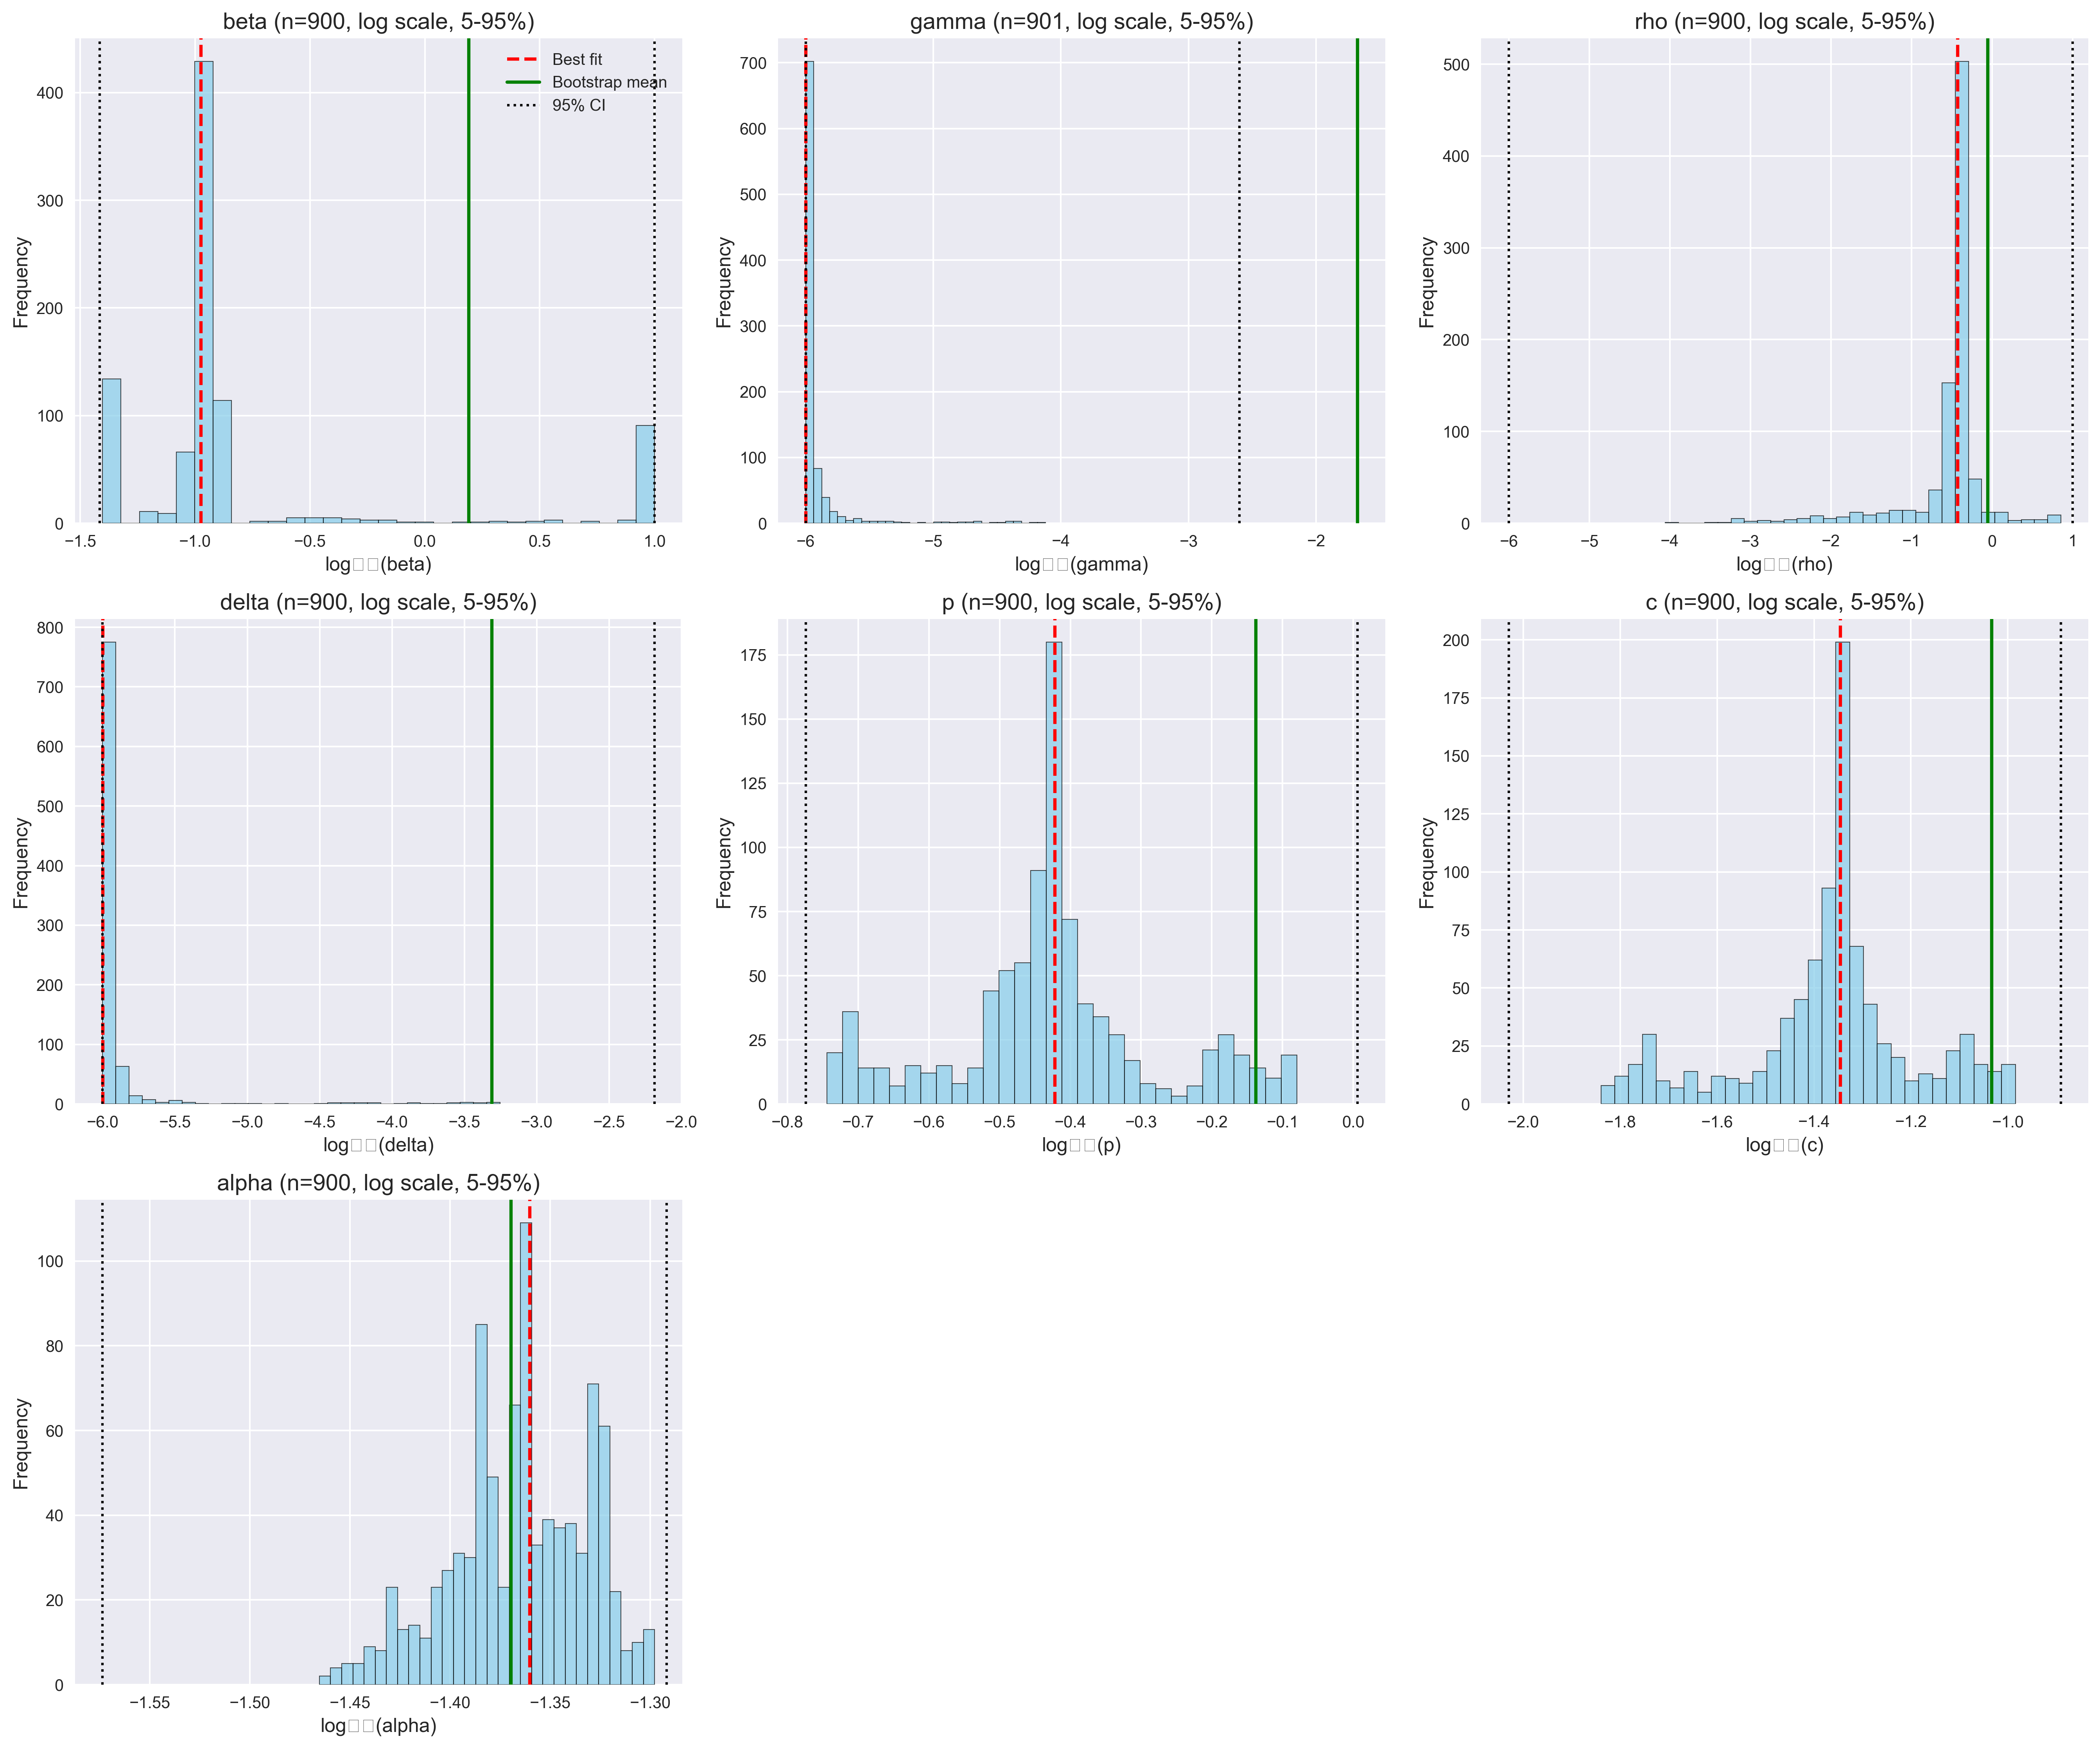
\includegraphics[width=\textwidth]{Plots/h5n1(2022)/tracheal/bootstrap_results/h5n1(2022)_tracheal_param_distributions.png}
\caption{Corner plot showing bootstrap parameter distributions for H5N1$_{2022}$ tracheal tissue (Model 3). Note: As discussed in the main text, this dataset exhibited numerical challenges during bootstrap analysis, with 21.4\% of bootstrap optimizations failing.}
\label{fig:h5n1_2022_tracheal_corner}
\end{figure}

\newpage
%------------------------------------------------------------------
\subsection{H5N1 (2022) - Tracheal Tissue (Alternative Analysis)}
%------------------------------------------------------------------

An alternative analysis was performed for H5N1$_{2022}$ tracheal tissue to address numerical challenges identified in the standard bootstrap analysis.

\subsubsection{Parameter Estimates}
\begin{table}[H]
\centering
\caption{Bootstrap parameter estimates for H5N1$_{2022}$ tracheal tissue - Alternative analysis (Model 3). Values represent mean estimates with 95\% confidence intervals from 1000 successful bootstrap resamples.}
\begin{tabular}{lccc}
\toprule
\textbf{Parameter} & \textbf{Mean} & \textbf{95\% CI Lower} & \textbf{95\% CI Upper} \\
\midrule
$\beta$ & 1.5223 & 0.0382 & 10.0000 \\
$\delta$ & 0.0020 & $<$0.0001 & 0.0032 \\
$p$ & 0.9717 & $<$0.0001 & 9.9991 \\
$c$ & 0.0006 & $<$0.0001 & 0.0066 \\
$\gamma$ & 0.8008 & 0.1658 & 0.9470 \\
$\rho$ & 0.1037 & 0.0090 & 0.1132 \\
$\alpha$ & 0.0425 & 0.0311 & 0.0508 \\
\bottomrule
\end{tabular}
\label{tab:h5n1_2022_trachealv1_params}
\end{table}

\subsubsection{Parameter Distribution Corner Plot}
\begin{figure}[H]
\centering
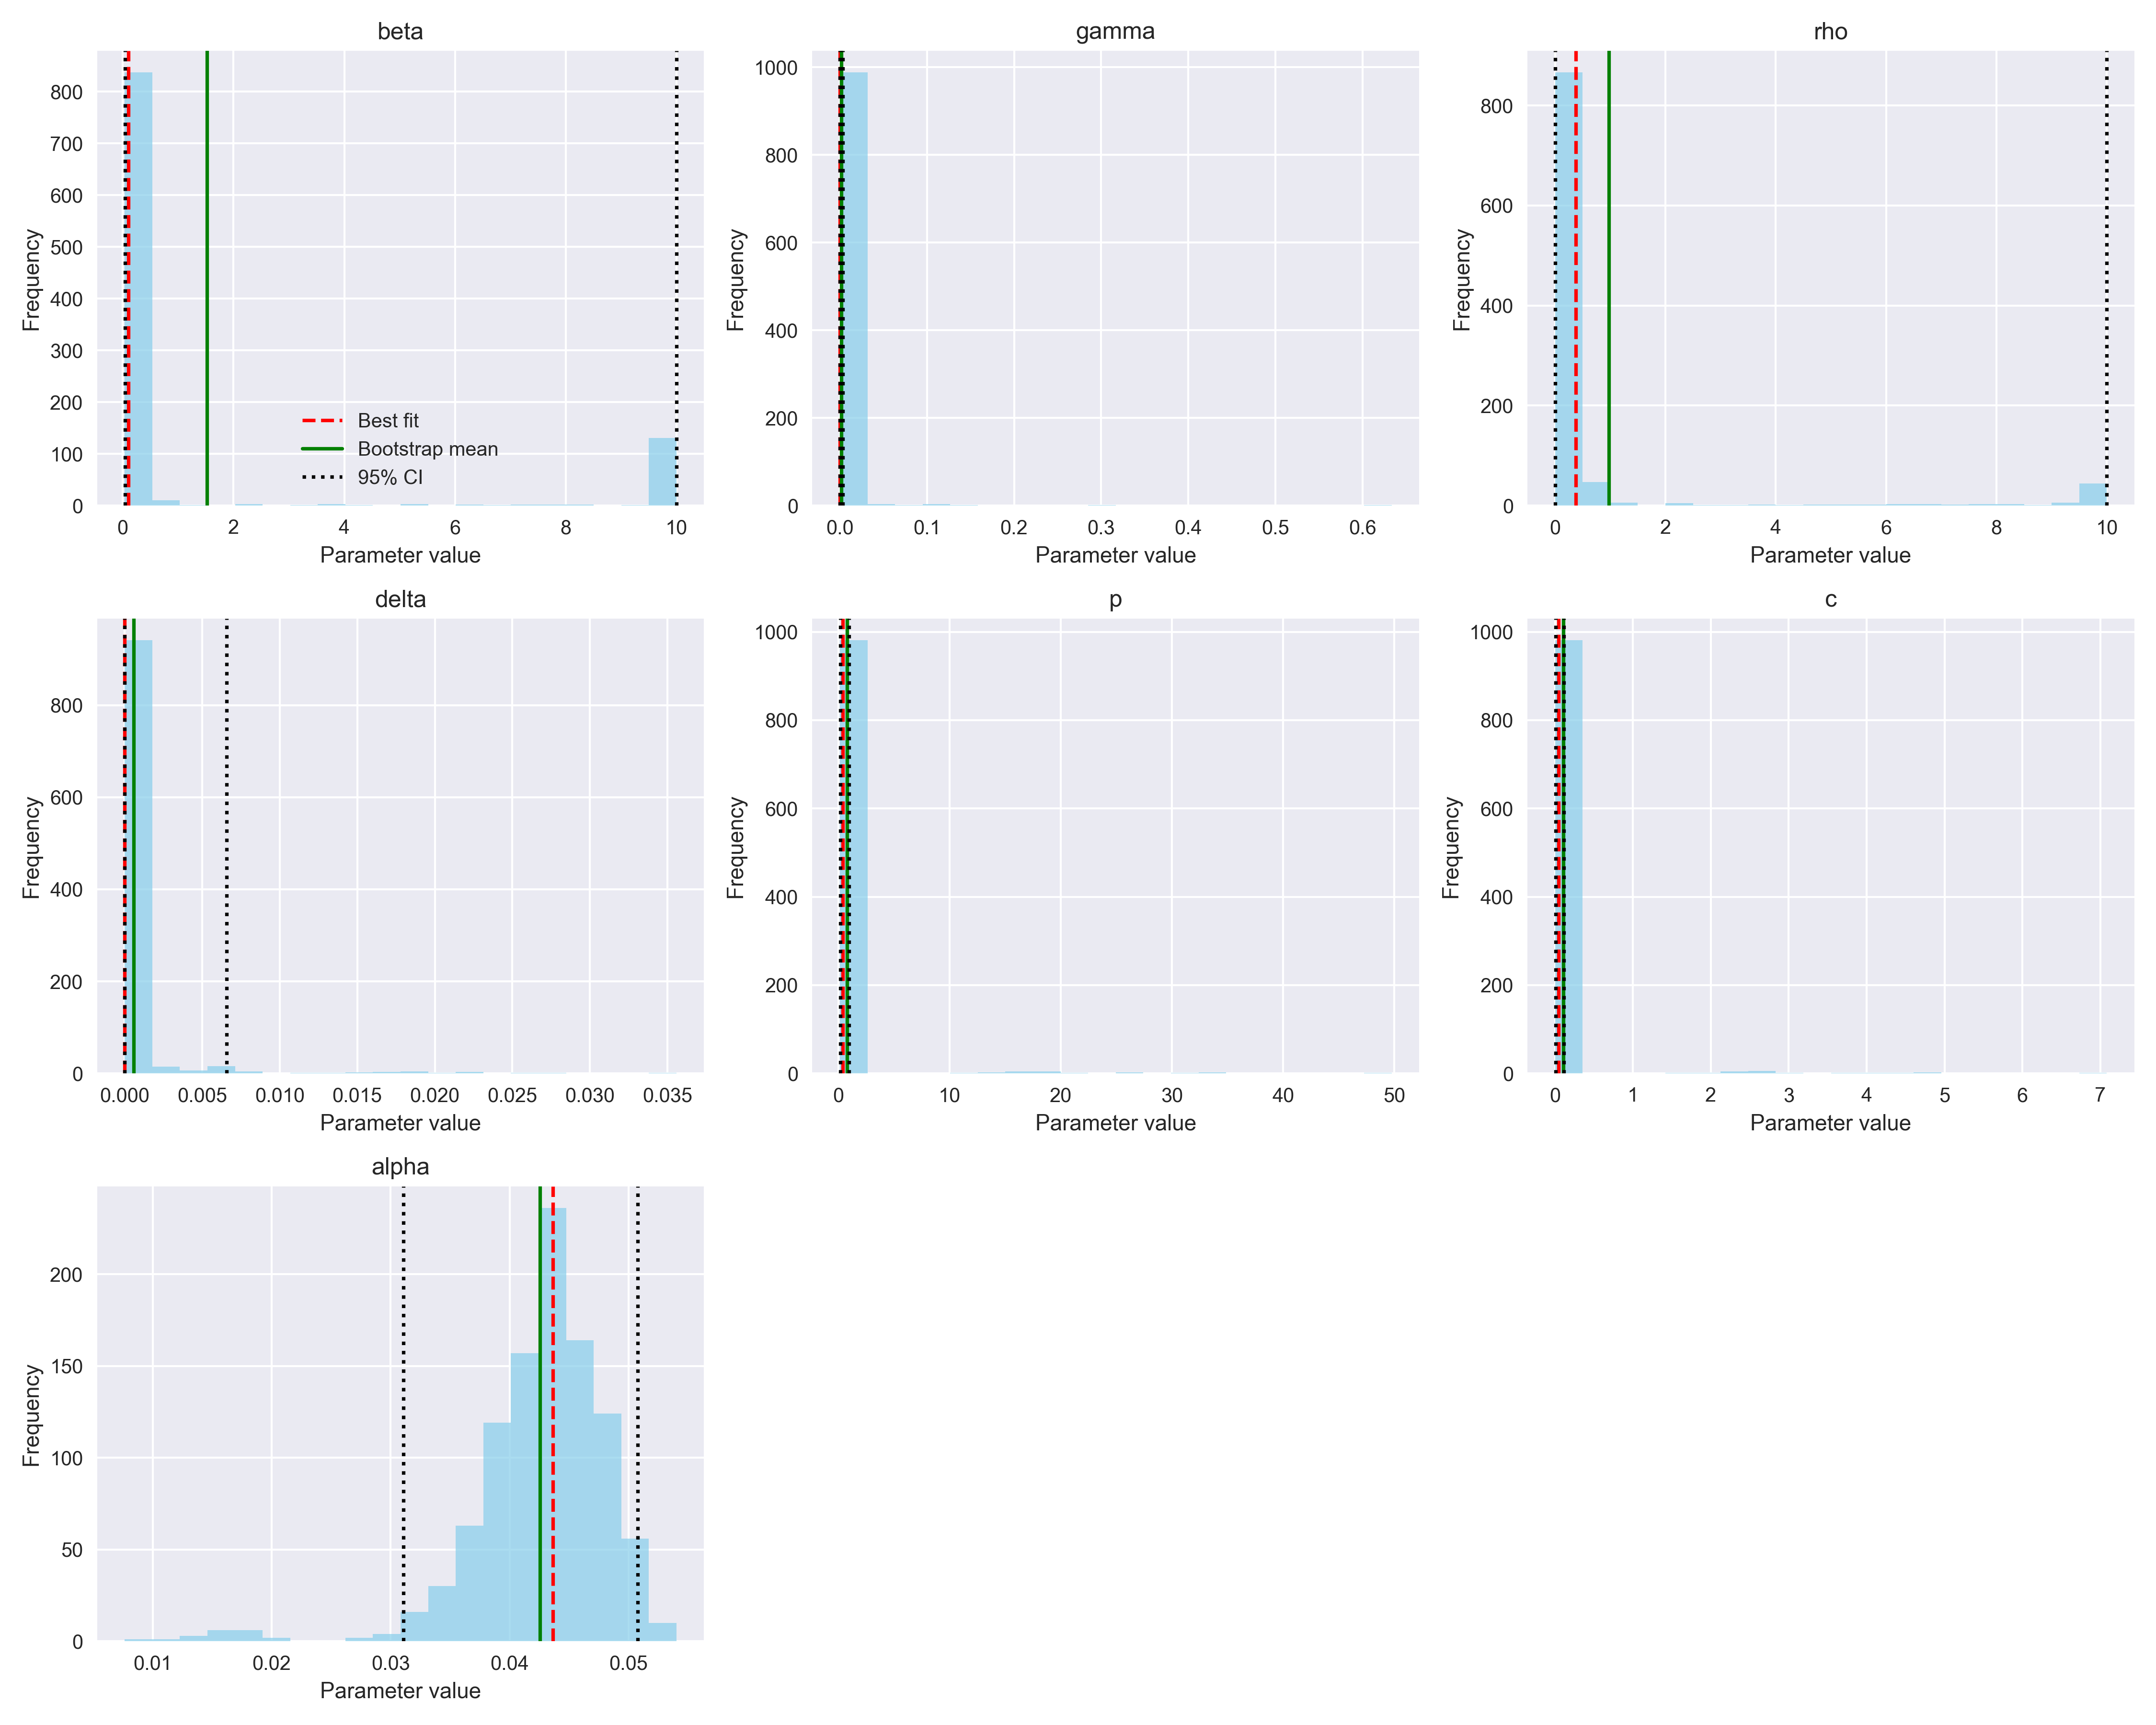
\includegraphics[width=\textwidth]{Plots/h5n1(2022)/trachealv1/bootstrap_results/h5n1(2022)_tracheal_param_distributions.png}
\caption{Corner plot showing bootstrap parameter distributions for H5N1$_{2022}$ tracheal tissue - Alternative analysis (Model 3). This analysis continued bootstrap resampling until 1000 successful fits were obtained (78.6\% success rate).}
\label{fig:h5n1_2022_trachealv1_corner}
\end{figure}

\newpage
%%%%%%%%%%%%%%%%%%%%%%%%%%%%%%%%%%%%%%%%%%%%%%%%%%%%%%%%%%%%%%%%%%%%%%%
\section{Summary of Key Findings}
%%%%%%%%%%%%%%%%%%%%%%%%%%%%%%%%%%%%%%%%%%%%%%%%%%%%%%%%%%%%%%%%%%%%%%%

\subsection{Strain-Specific Differences}
The bootstrap parameter estimates reveal several key patterns:

\begin{itemize}
    \item \textbf{Interferon Response Rate ($\gamma$):} H5N1$_{2022}$ demonstrates higher $\gamma$ values (0.73-0.80 day$^{-1}$ in tracheal tissue) compared to H5N1$_{2005}$ (0.26-0.29 day$^{-1}$), indicating stronger interferon-induced protection in the recent clade.
    
    \item \textbf{Refractory State Duration:} The inverse of $\rho$ represents the mean duration cells remain in the refractory state. H5N1$_{2022}$ shows longer refractory periods, consistent with more sustained antiviral protection.
    
    \item \textbf{Tissue-Specific Patterns:} Nasal tissue consistently shows different parameter profiles than tracheal tissue across all strains, with implications for understanding differential viral replication in upper versus lower respiratory tract.
\end{itemize}

\subsection{Parameter Uncertainty and Identifiability}
Several parameters show wide confidence intervals, particularly:
\begin{itemize}
    \item Parameters near boundary values (0 or 10) suggest potential structural identifiability issues
    \item H3N2$_{2003}$ tracheal tissue shows exceptionally high $\gamma$ values with wide confidence intervals
    \item H5N1$_{2022}$ tracheal analysis required special handling due to numerical challenges
\end{itemize}

These findings highlight the importance of comprehensive uncertainty quantification in mathematical modeling of viral dynamics and underscore the need for careful interpretation of parameter estimates in the context of biological plausibility.

\end{document}